\documentclass[
	a4paper,
	oneside,
	DIV = 12,
	fontsize = 13pt,
	headings = normal,
]{scrartcl}

%%% Page geometry and precise margins
\usepackage[
	pass,
	left   = 20mm,
	top    = 15mm,
	right  = 10mm,
	bottom = 15mm,
]{geometry}
%%%

%%% Length calculations
\usepackage{calc}
%%%

%%% Support for color
\usepackage{xcolor}
\definecolor{lightblue}{HTML}{03A9F4}
\definecolor{red}{HTML}{F44336}
%%%

%%% Including graphics
\usepackage{graphicx}
%%%

%%% Font selection
\usepackage{fontspec}

\setromanfont{STIX Two Text}[
	SmallCapsFeatures = {LetterSpace = 5},
]

\setsansfont{IBM Plex Sans}[
	Scale = MatchUppercase,
]

\setmonofont{IBM Plex Mono}[
	Scale = MatchUppercase,
]
%%%

%%% Math typesetting
\usepackage{amsmath}

\usepackage{unicode-math}
\setmathfont{STIX Two Math}
%%%

%%% List settings
\usepackage{enumitem}
\setlist[enumerate]{
	label*      = {\arabic*.},
	leftmargin  = *,
	labelindent = \parindent,
	topsep      = 1\baselineskip,
	parsep      = 0\baselineskip,
	itemsep     = 1\baselineskip,
}

\setlist[itemize]{
	label*      = {—},
	leftmargin  = *,
	labelindent = \parindent,
	topsep      = 1\baselineskip,
	parsep      = 0\baselineskip,
	itemsep     = 1\baselineskip,
}

\setlist[description]{
	font        = {\rmfamily\upshape\bfseries},
	topsep      = 1\baselineskip,
	parsep      = 0\baselineskip,
	itemsep     = 0\baselineskip,
}

%%%

%%% Structural elements typesetting
\setkomafont{pagenumber}{\rmfamily}
\setkomafont{disposition}{\rmfamily\bfseries}

% Sectioning
\RedeclareSectionCommand[
	beforeskip = -1\baselineskip,
	afterskip  = 1\baselineskip,
	font       = {\normalsize\bfseries\scshape},
]{section}

\RedeclareSectionCommand[
	beforeskip = -1\baselineskip,
	afterskip  = 1\baselineskip,
	font       = {\normalsize\bfseries},
]{subsection}

\RedeclareSectionCommand[
	beforeskip = -1\baselineskip,
	afterskip  = 1\baselineskip,
	font       = {\normalsize\bfseries},
]{subsubsection}
%%%

%%% Typographic enhancements
\usepackage{microtype}
%%%

%%% Language-specific settings
\usepackage{polyglossia}
\setmainlanguage{ukrainian}
\setotherlanguages{english}
%%%

%%% Captions
\usepackage{caption}
\usepackage{subcaption}

%\DeclareCaptionLabelFormat{closing}{#2)}
%\captionsetup[subtable]{labelformat = closing}

%\captionsetup[subfigure]{labelformat = closing}

\captionsetup[table]{
	aboveskip = 0\baselineskip,
	belowskip = 1\baselineskip,
}

\captionsetup[figure]{
	aboveskip = 1\baselineskip,
	belowskip = 0\baselineskip,
}

\captionsetup[subfigure]{
	aboveskip = 0.25\baselineskip,
	belowskip = 0\baselineskip,
}

\captionsetup[subfigure]{
	labelformat = simple,
	labelformat = brace,
}
%%%

%%% Table typesetting
\usepackage{booktabs}
\usepackage{longtable}

\usepackage{multirow}

\usepackage{array}
\newcolumntype{v}[1]{>{\raggedright\arraybackslash\hspace{0pt}}p{#1}}
\newcolumntype{b}[1]{>{\centering\arraybackslash\hspace{0pt}}p{#1}}
\newcolumntype{n}[1]{>{\raggedleft\arraybackslash\hspace{0pt}}p{#1}}
%%%

%%% Dingbats
\usepackage{pifont}
%%%

%%% Links and hyperreferences
\usepackage{hyperref}
\hypersetup{
	bookmarksnumbered = true,
	colorlinks      = false,
	linkbordercolor = red,
	urlbordercolor  = lightblue,
	pdfborderstyle  = {/S/U/W 1.5},
}
%%%

%%% Length adjustments
% Set baselineskip to ~15pt, default is 14.5pt
% \linespread{1.034483}
% \linespread{1.068966} % ~15.5pt
\setlength{\emergencystretch}{1em}
\setlength{\parindent}{1.5em}
\newlength{\gridunitwidth}
\setlength{\gridunitwidth}{\textwidth / 12}
\setlength{\floatsep}{1\baselineskip}
\setlength{\intextsep}{1\baselineskip}
\setlength{\textfloatsep}{1\baselineskip}
%%%

%%% Custom commands
\newcommand{\allcaps}[1]{{\addfontfeatures{LetterSpace = 5}#1}}
\newcommand{\progname}[1]{\texttt{#1}}

\newcommand{\CheckMark}{\ding{51}}
\newcommand{\Mytextrightarrow}{$\rightarrow$\hspace{0.25em}}
%%%

%%% Make typography adhere to made-up standards
\PolyglossiaSetup{ukrainian}{indentfirst = true}

% Sectioning
\RedeclareSectionCommand[
	beforeskip = -1\baselineskip,
	afterskip  = 1\baselineskip,
	indent     = 12.5mm,
	font       = {\normalsize\bfseries},
]{section}

\RedeclareSectionCommand[
	beforeskip = -1\baselineskip,
	afterskip  = 1\baselineskip,
	indent     = 12.5mm,
	font       = {\normalsize\bfseries},
]{subsection}

\RedeclareSectionCommand[
	beforeskip = -1\baselineskip,
	afterskip  = 1\baselineskip,
	indent     = 12.5mm,
	font       = {\normalsize\bfseries},
]{subsubsection}

\setlength{\parindent}{12.5mm}

\usepackage{leading}
\leading{21pt}

%%%

\begin{document}
	\newgeometry{
		left   = 20mm,
		top    = 15mm,
		right  = 10mm,
		bottom = 15mm,
		footskip = \baselineskip, % reduce footer vertical skip so page numbers are visible
	}
	\begin{titlepage}
		\begin{center}
			Міністерство освіти і науки України\\
			Національний авіаційний університет\\
			Навчально-науковий інститут комп'ютерних інформаційних технологій\\
			Кафедра комп'ютеризованих систем управління

			\vspace{\fill}
				Лабораторна робота №2\\
				з дисципліни «Діагностика та експлуатація комп'ютера»\\
				на тему «Дефрагментація жорсткого диску»\\

			\vspace{\fill}

			\begin{flushright}
				Виконав:\\
				студент \allcaps{ННІКІТ}\\
				групи СП-325\\
				Клокун В.\,Д.\\
				Перевірив:\\
				Масловський Б.\,Г.
			\end{flushright}

			Київ 2018
		\end{center}
	\end{titlepage}

	\section{Ціль роботи}
		Ознайомлення з~процесом дефрагментації жорсткого диску.

	\section{Короткі теоретичні відомості}
		Під час запису файлу на~жорсткий диск існує імовірність, що файл не~поміститься у~відведений йому простір і~операційна система розділить його на~логічні частини. Такий поділ файлу на~частини і~називається фрагментацією файлу. Фрагментацією диска або~файлової системи називають відсоток фрагментованих файлів.

		Найбільш сильно фрагментуються файли, які часто змінюють розмір, наприклад, бази даних і~протоколи (логи) програм, а~також файли великого розміру, наприклад, фільми.

		Чим сильніше фрагментована файлова система, тим повільніше комп'ютер працює з~інформацією на~жорсткому диску. А~в~зв'язку з~тим, що~жорсткий диск~— одне з~найбільш вузьких місць у~швидкодії~ПК, то~при~збільшенні фрагментації може значно страждати продуктивність всього комп'ютера.

		Варто звернути увагу на~те, що~чим сильніше заповнений жорсткий диск, тим сильніше заповнений диск, тим сильніше починають фрагментуватися файли на~ньому. Щоб не~доводити фрагментованість до~критичного рівня не~заповнюйте розділ жорсткого диска більш ніж~на~80\%.

		Дефрагментацією комп'ютера називається процес під~час якого прибираються фрагменти файлів або~хоча~б зменшується їх~кількість.

	\section{Хід роботи}
		Запускаємо \textenglish{VMware Player} та~віртуальну машину з~встановленою операційіною системою \textenglish{Windows~XP}.

		\subsection{Дефрагментація засобами операційної системи~\textenglish{Windows XP}}
				Виконуємо дефрагментацію диску засобами \textenglish{Windows XP}~(рис.~\ref{fig:01-winxp-defrag}). Для цього запускаємо утиліту~\textenglish{Disk Defragmenter~(Start~\Mytextrightarrow All Programs~\Mytextrightarrow Acessories~\Mytextrightarrow Disk Defragmenter)}. Натискаємо кнопку~\textenglish{«Analyze»} для~виконання аналізу диску, а~потім~— кнопку~\textenglish{«Defragment»} для~виконання дефрагментації.
			\begin{figure}[!htbp]
				\centering
				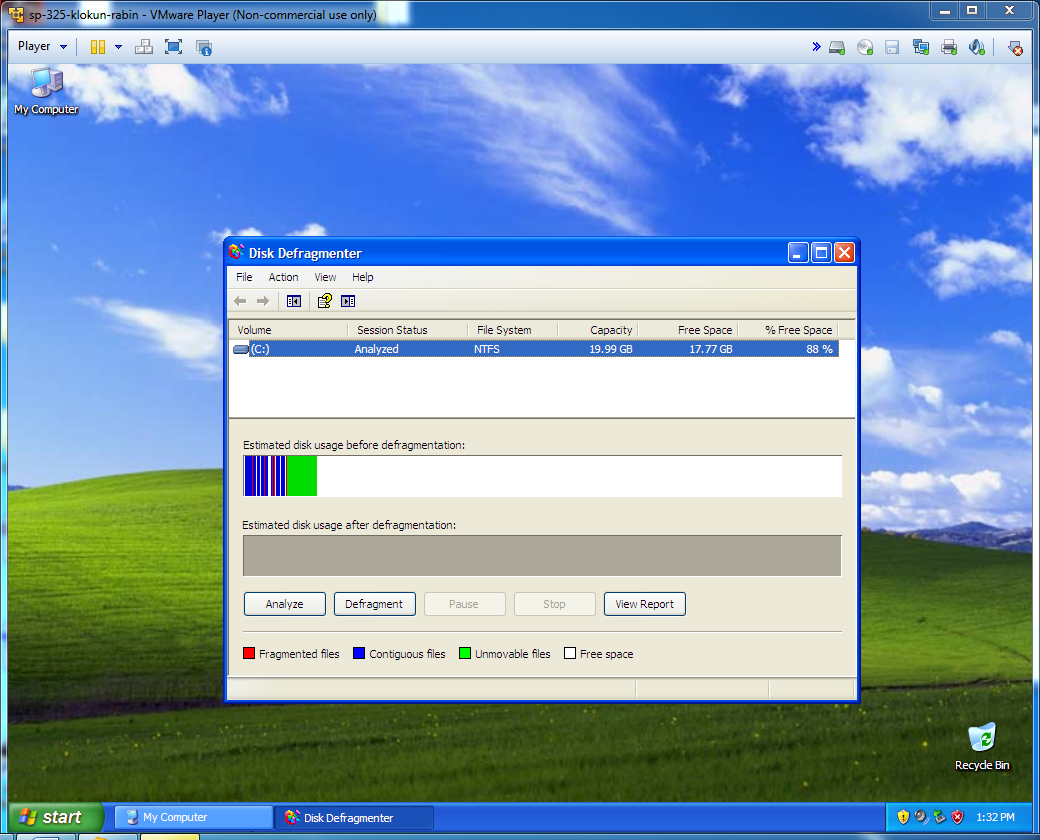
\includegraphics[height = 8\baselineskip]{./assets/lab-02-01.png}
				\caption{Результат дефрагментації диску засобами \textenglish{Windows~XP}}
				\label{fig:01-winxp-defrag}
			\end{figure}

		Копіюємо сторонні утиліти для~виконання дефрагментаціїї на~жорсткий диск. Для цього монтуємо образ диску, який знаходиться в~папці з~лабораторною роботою, у~віртуальну машину.

		\subsection{Дефрагментація засобами програми~\textenglish{Defraggler}}
			Виконуємо дефрагментацію програмою \textenglish{Defraggler}~(рис.~\ref{fig:02-defraggler-defrag}). Для цього запускаємо її та~натискаємо на~кнопку~\textenglish{«Defrag»}.
			\begin{figure}[!htbp]
				\centering
				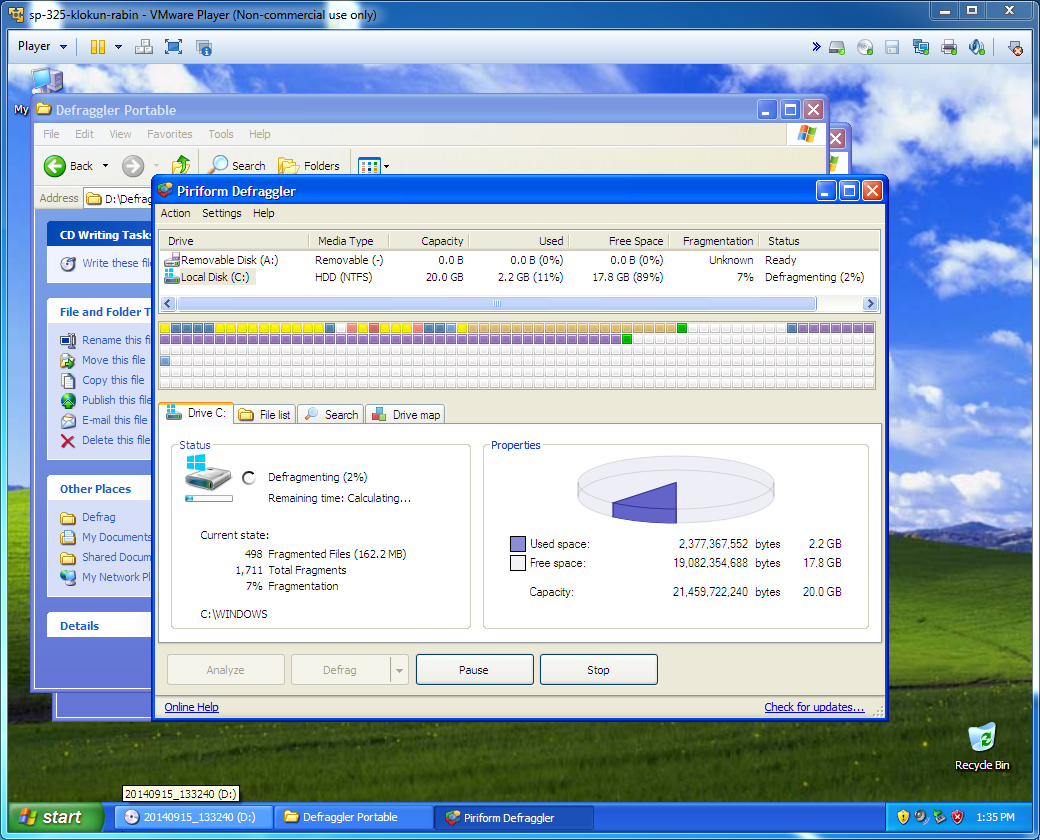
\includegraphics[height = 8\baselineskip]{./assets/lab-02-03.png}
				\caption{Результат дефрагментації диску засобами програми \textenglish{Defraggler}}
				\label{fig:02-defraggler-defrag}
			\end{figure}

		\subsection{Дефрагментація засобами програми~\textenglish{Vopt}}
			Виконуємо дефрагментацію програмою \textenglish{Vopt}~(рис.~\ref{fig:03-vopt-defrag}). Для цього запускаємо її та~натискаємо на~кнопку~\textenglish{«Defrag drive»}.
			\begin{figure}[!htbp]
				\centering
				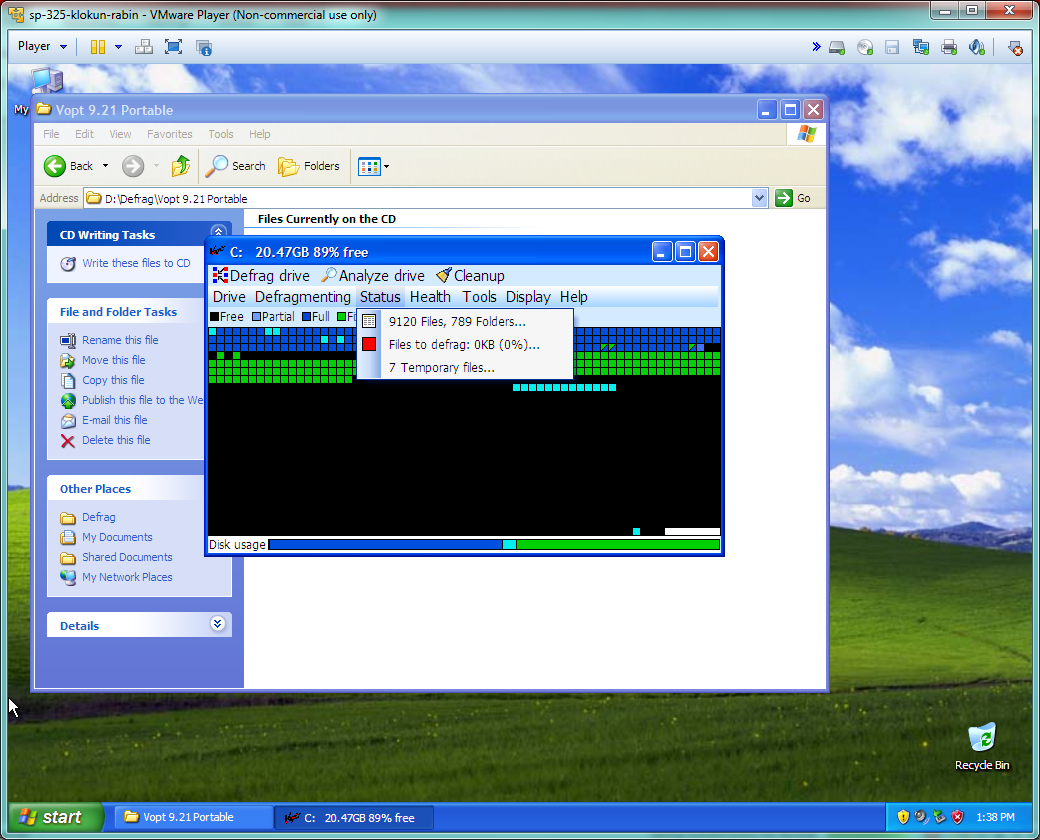
\includegraphics[height = 8\baselineskip]{./assets/lab-02-04.png}
				\caption{Результат дефрагментації диску засобами програми \textenglish{Vopt}}
				\label{fig:03-vopt-defrag}
			\end{figure}

		\subsection{Дефрагментація засобами програми~\textenglish{Auslogics Disk Defrag}}
			Виконуємо дефрагментацію програмою \textenglish{Auslogics Disk Defrag}~(рис.~\ref{fig:04-auslogics-defrag}). Для цього запускаємо її та~натискаємо на~кнопку~\textenglish{«Defrag»}.
			\begin{figure}[!htbp]
				\centering
				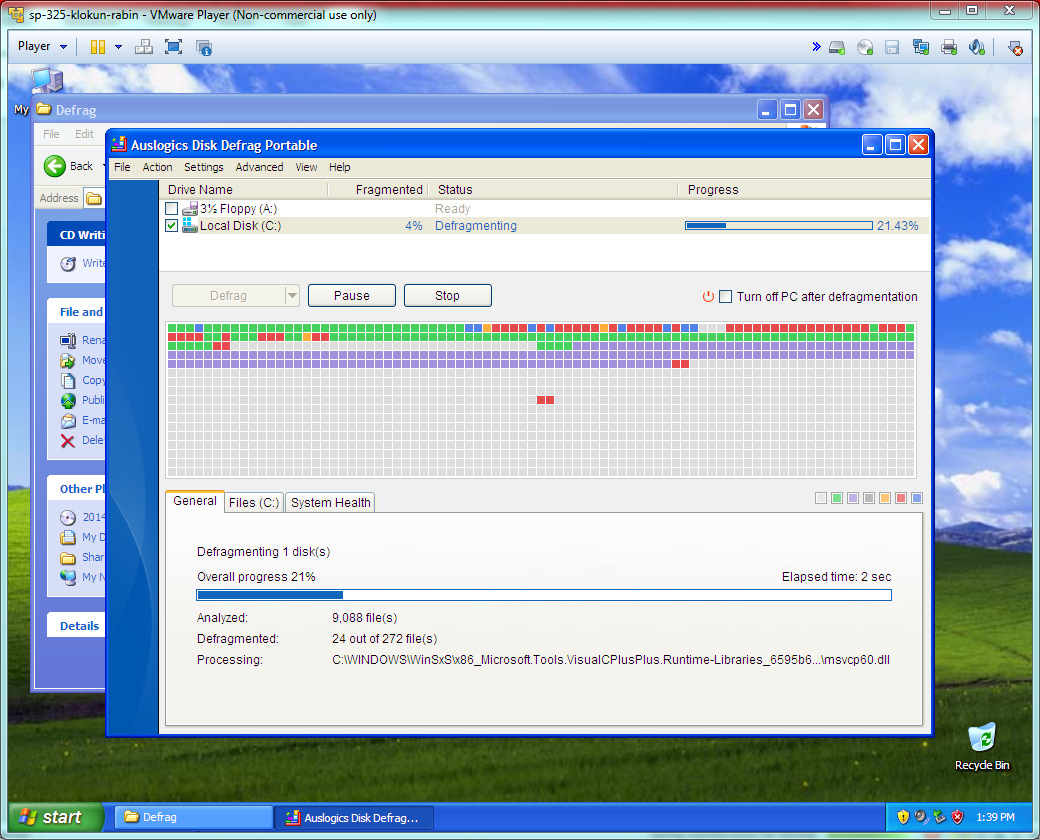
\includegraphics[height = 8\baselineskip]{./assets/lab-02-05.png}
				\caption{Результат дефрагментації диску засобами програми \textenglish{Auslogics Disk Defrag}}
				\label{fig:04-auslogics-defrag}
			\end{figure}

		\subsection{Дефрагментація засобами програми~\textenglish{O\&O Defrag}}
			Виконуємо дефрагментацію програмою \textenglish{O\&O Defrag}~(рис.~\ref{fig:05-o-et-o-defrag}). Для цього запускаємо її, розгортаємо вікно програми на~повний екран та~натискаємо на~кнопку~\textenglish{«Start»}.
			\begin{figure}[!htbp]
				\centering
				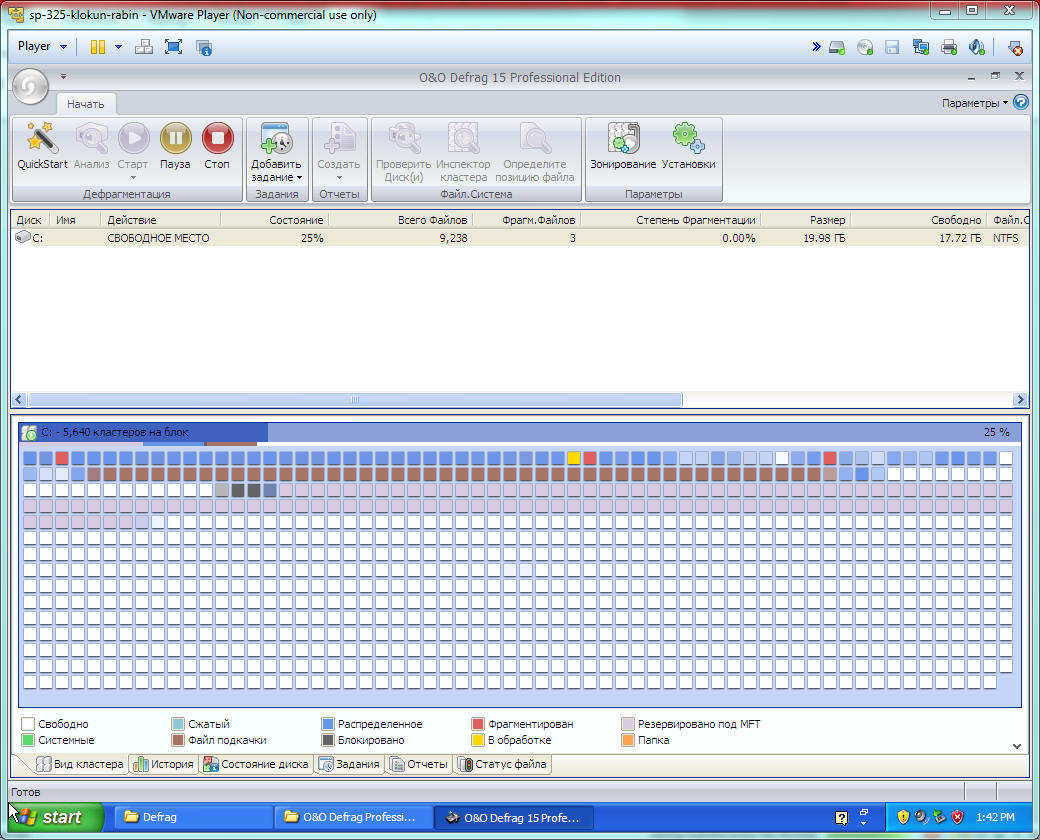
\includegraphics[height = 8\baselineskip]{./assets/lab-02-06.png}
				\caption{Результат дефрагментації диску засобами програми \textenglish{O\&O Defrag}}
				\label{fig:05-o-et-o-defrag}
			\end{figure}

		\subsection{Дефрагментація засобами програми~\textenglish{Ultimate Defrag}}
			Виконуємо дефрагментацію програмою \textenglish{Ultimate Defrag}~(рис.~\ref{fig:06-ultimate-defrag}). Для цього запускаємо її, розгортаємо вікно програми на~повний екран та~натискаємо на~кнопку~\textenglish{«Start»}.
			\begin{figure}[!htbp]
				\centering
				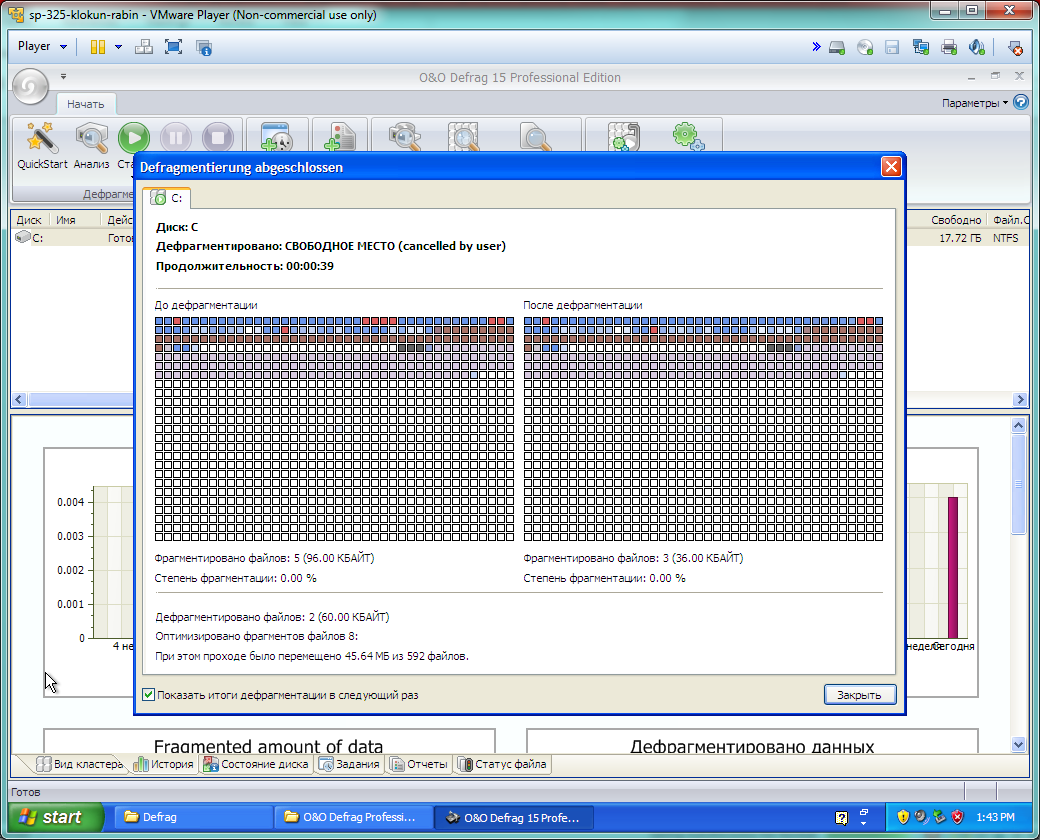
\includegraphics[height = 8\baselineskip]{./assets/lab-02-07.png}
				\caption{Результат дефрагментації диску засобами програми \textenglish{Ultimate Defrag}}
				\label{fig:06-ultimate-defrag}
			\end{figure}

	\section{Домашнє завдання}
		Домашнім завданням даної лабораторної роботи є проведення дефрагментації жорстких дисків на власному комп'ютері~(результати виконання на~рис.~\ref{fig:homework}).
		\begin{figure}[!htbp]
			\begin{subfigure}{0.5\textwidth}
				\centering
				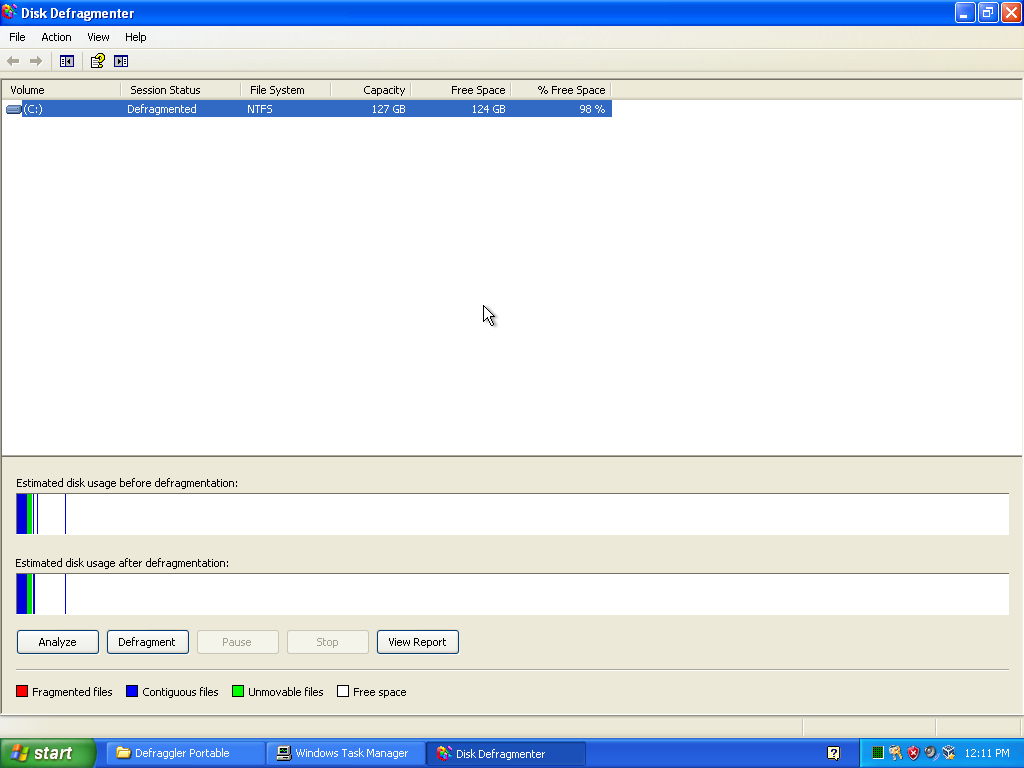
\includegraphics[height = 8\baselineskip]{./assets/lab-02-hw-01.png}
				\caption{}
				\label{subfig:homework-01}
			\end{subfigure}%
			\begin{subfigure}{0.5\textwidth}
				\centering
				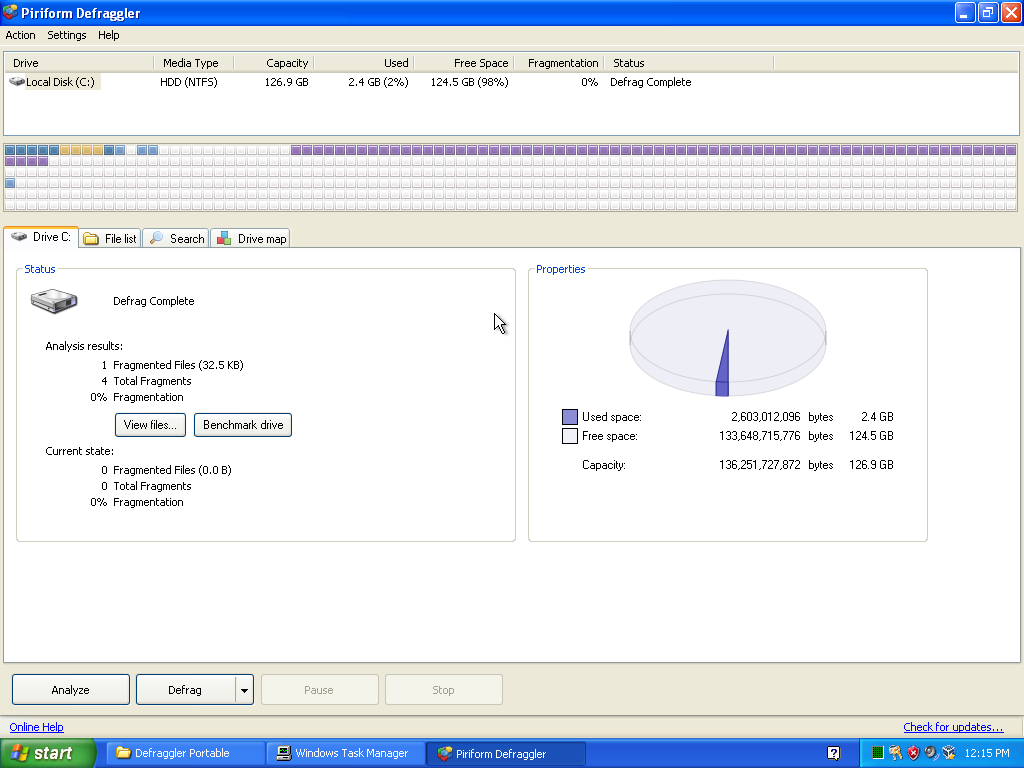
\includegraphics[height = 8\baselineskip]{./assets/lab-02-hw-02.png}
				\caption{}
				\label{subfig:homework-02}
			\end{subfigure}%
			\vspace*{\floatsep}
			\begin{subfigure}{0.5\textwidth}
				\centering
				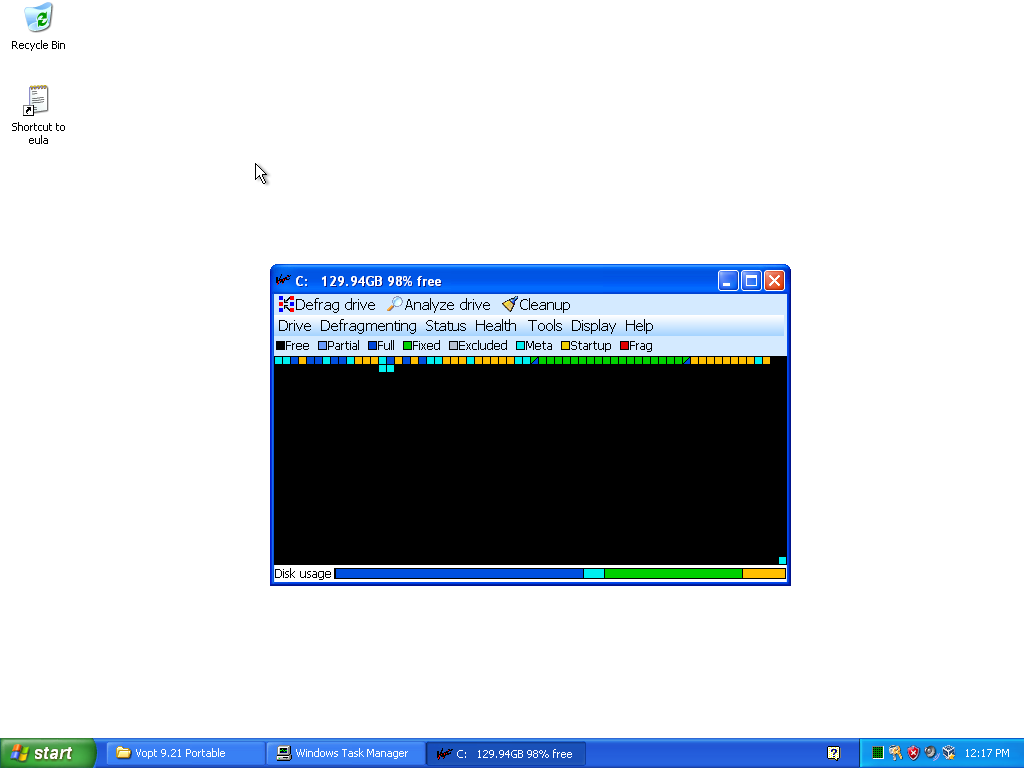
\includegraphics[height = 8\baselineskip]{./assets/lab-02-hw-03.png}
				\caption{}
				\label{subfig:homework-03}
			\end{subfigure}%
			\begin{subfigure}{0.5\textwidth}
				\centering
				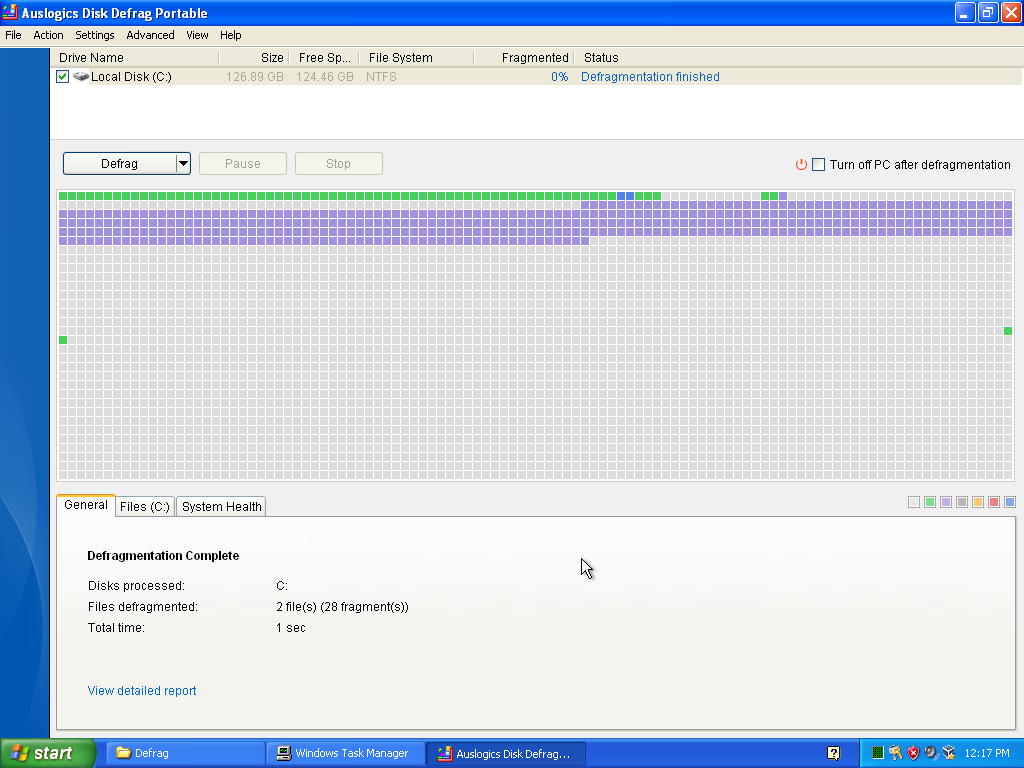
\includegraphics[height = 8\baselineskip]{./assets/lab-02-hw-04.png}
				\caption{}
				\label{subfig:homework-04}
			\end{subfigure}%
			\vspace*{\floatsep}
			\begin{subfigure}{0.5\textwidth}
				\centering
				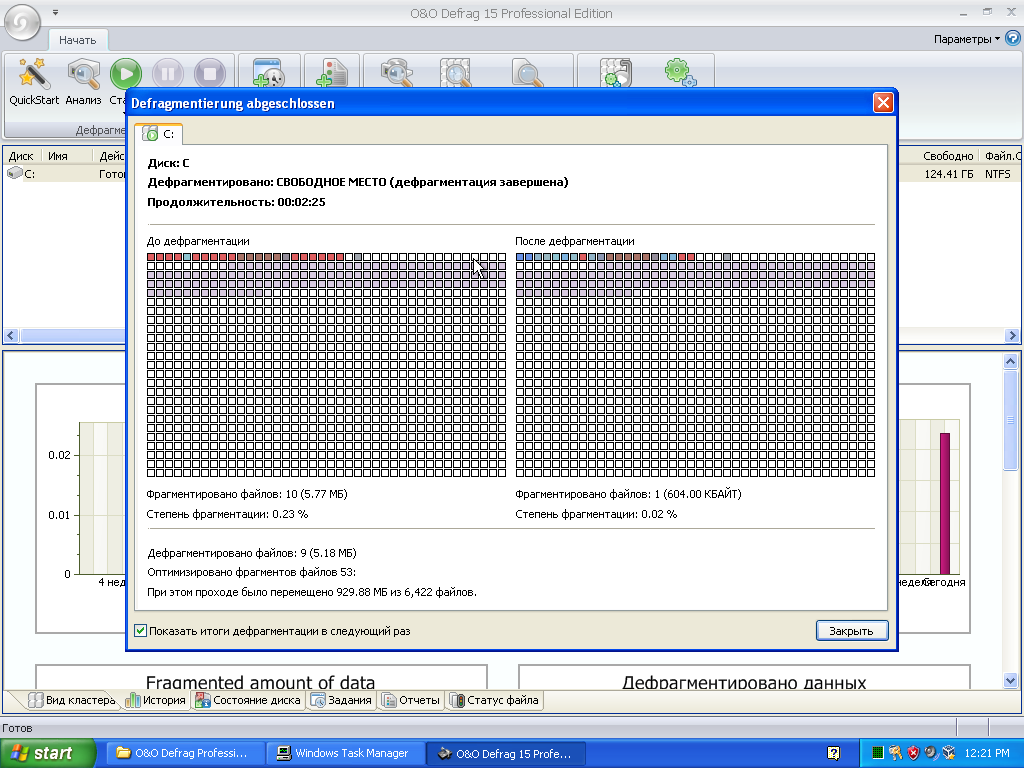
\includegraphics[height = 8\baselineskip]{./assets/lab-02-hw-05.png}
				\caption{}
				\label{subfig:homework-05}
			\end{subfigure}%
			\begin{subfigure}{0.5\textwidth}
				\centering
				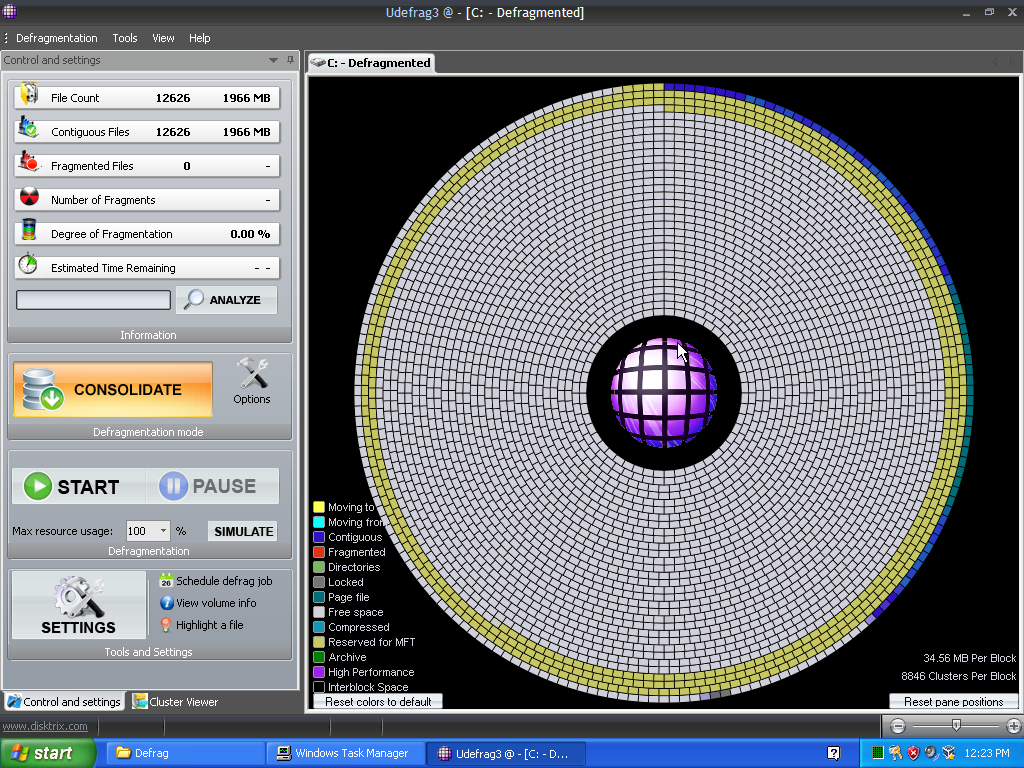
\includegraphics[height = 8\baselineskip]{./assets/lab-02-hw-06.png}
				\caption{}
				\label{subfig:homework-06}
			\end{subfigure}%
			\caption{Результати виконання домашнього завдання: \subref{subfig:homework-01}~— \textenglish{Disk Defragmenter}, \subref{subfig:homework-02}~— \textenglish{Defraggler}, \subref{subfig:homework-03}~— \textenglish{Vopt}, \subref{subfig:homework-04}~— \textenglish{Auslogics Disk Defrag}, \subref{subfig:homework-05}~— \textenglish{O\&O~Defrag}, \subref{subfig:homework-06}~— \textenglish{Ultimate Defrag}}
			\label{fig:homework}
		\end{figure}

	\section{Висновок}
		Виконуючи дану лабораторну роботу, ми~ознайомились з~процесом дефрагментації жорстких дисків на~прикладі стандартної програми операційної системи \textenglish{Windows~XP}, а~також сторонніх програм \textenglish{Defraggler, Vopt, Auslogics Disk Defrag, O\&O Defrag,~Ultimate Defrag}.

\end{document}
